\label{sec:dbb:results}

\section{Morphology characterization and coefficient of restitution evolution during discharge}
As an alkaline battery is discharged, the anode undergoes oxidation from Zn to ZnO, as seen in Eq.~\ref{eq:zn1} and~\ref{eq:zn2}, while the cathode is reduced from {\ce{MnO_2}} to MnOOH, shown in Eq.~\ref{eq:mn}.

\begin{equation}
{\ce{Zn + 4OH^- -> Zn(OH)^{2-}_{4} + 2e^-}}
\label{eq:zn1}
\end{equation}
\begin{equation}
{\ce{Zn(OH)^{2-}_{4} -> ZnO + H_{2}O + 2OH^-}}
\label{eq:zn2}
\end{equation}
\begin{equation}
{\ce{MnO_{2} + H_{2}O + e- -> MnOOH + OH^-}}
\label{eq:mn}
\end{equation}

\noindent Equation~\ref{eq:zn1} shows that the battery produces {\ce{Zn(OH)^{2-}_{4}} ions in solution until the electrolyte becomes supersaturated, at which point it begins to precipitate as ZnO ~\cite{linden}.

\textit{Post mortem} analysis shows that in alkaline AA batteries, the Zn gel anode initially exists as discrete Zn particles in a matrix of KOH electrolyte and a gelling agent. After discharge, the anode densifies into a porous ZnO solid that appears more compact closer to the separator, as shown in Fig.~\ref{fig:SEM}. The densification of the anode affects the mechanical properties of the battery. The COR, which measures the elasticity of a collision between two objects, is one such mechanical property that can be determined as shown in Eq.~\ref{eq:cor}.



\begin{figure}[htb]
  \centering
    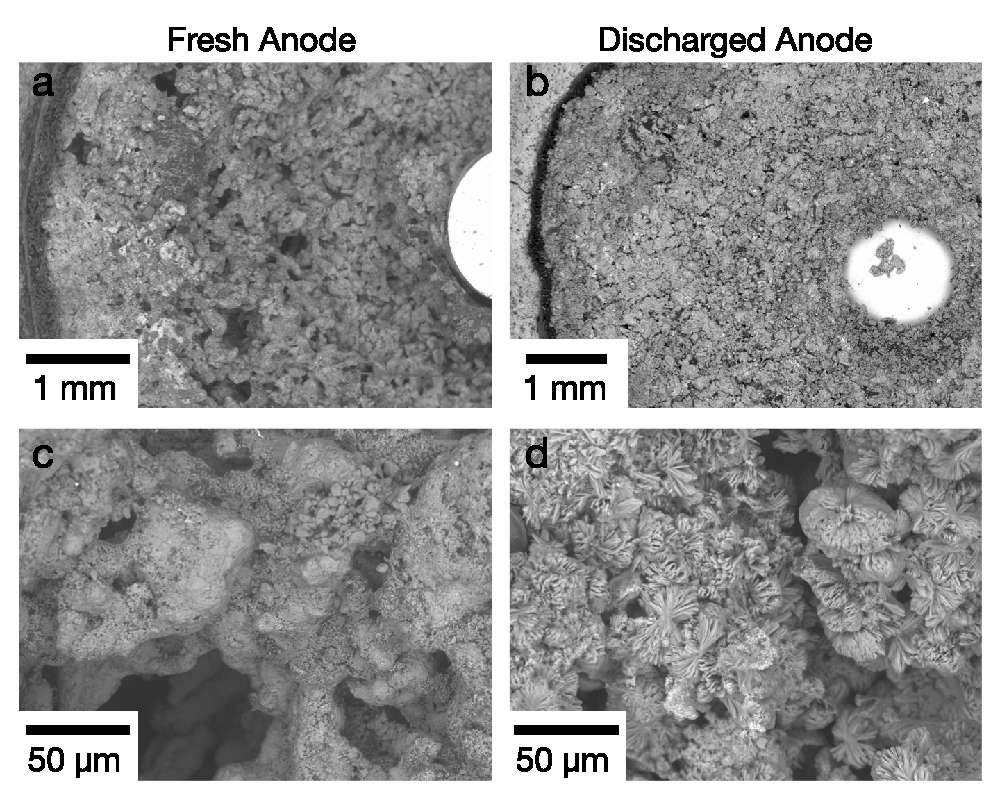
\includegraphics[width=0.8\textwidth]{ch3-dbb/Images/ZnSEM.eps}
    \caption[SEM images of sectioned fresh and fully discharged alkaline batteries]{a) SEM image of ``fresh" cell. b) SEM image of the same cell after full discharge (2850 mAh passed). c) High mag. SEM image showing fresh Zn particles. d) High mag. SEM image showing coagulated ZnO particles after full discharge.}
    \label{fig:SEM}
\end{figure}

\begin{equation}
COR = \frac{1}{N} \sum\limits_{n=1}^N \sqrt{\frac{h_{n+1}}{h_n}}
\label{eq:cor}
\end{equation}

\noindent where \(N\) is the number of bounces, and \(h\) denotes the bounce heights determined from Eq.~\ref{eq:bounce}. Using the bounce test described previously, the COR of alkaline batteries was measured through full discharge.

Figure~\ref{fig:COR1to3} shows the evolution of the COR for three identical AA cells as capacity is passed in increments of 280 milliamp-hours (mAh) at 280 mA, corresponding to a rate of C/10. The inset shows a composited image of the corresponding drop tests for a single cell. A sharp increase in COR occurs at 80\% SOC, when 560 mAh have passed, followed by asymptotic leveling of the COR at a value of 0.66\(\pm\) 0.02 after 50\% SOC (1400 mAh passed).  The three cells show excellent agreement in the low and high COR regimes, and the variance in the dynamic regime (80\% to 50\% SOC) shows that there is some variance from cell to cell in ZnO growth.

\clearpage

\begin{figure}[hbt]
  \centering
    \includegraphics[width=0.8\textwidth]{ch3-dbb/Images/cor280.pdf}
    \caption[Coefficient of restitution evolution at 280 mA.]{Coefficient of restitution as a function of capacity passed at 280 mA. Inset: Composited image of bounce behavior for a single cell over full depth of discharge}
    \label{fig:COR1to3}
\end{figure}

To show the transition between the low COR and high COR regimes more clearly and to gauge the effect of discharge rate on the COR evolution, cells were discharged at 50 mA in one hour intervals (50 mAh) prior to bounce testing, corresponding to a rate of roughly C/57. As shown in Figure~\ref{fig:50mah} the COR is constant for low depths of discharge, similar to the cells discharged at 280 mA. The rise in COR begins after 450 mAh have been passed, which is roughly 100 mAh earlier than in the cells discharged at 280 mA. The leveling of COR for these cells occurs at 950 mAh passed, which is roughly 450 mAh earlier than the saturation point for COR of cells discharged at 280 mA. It has been shown previously by Horn et al~\cite{horn} that lower discharge rates will result in a more even distribution of ZnO in the anode, compared to that of a higher discharge rate, thus a more even distribution of ZnO. We posit that because ZnO is the major contributor to the changes in mechanical properties of the battery, a more even distribution results in earlier leveling of the COR.

\begin{figure}[ht]
  \centering
    \includegraphics[width=0.8\textwidth]{ch3-dbb/Images/50mAh.eps}
    \caption[Coefficient of restitution evolution at 50 mA.]{Coefficient of restitution as a function of capacity passed at 50 mA in 50 mAh increments.}
    \label{fig:50mah}
\end{figure}


\section{Possible reasons for COR evolution}

As the stainless steel casing does not change or partake in the electrochemical reaction, four possible effects associated with discharging an alkaline battery may be correlated with the observed change in COR: 1) mass loss, 2) reduction of the cathode from {\ce{MnO_2}} to {\ce{MnOOH}}, 3) water consumption, and 4) oxidation of the anode from Zn to ZnO. We will discuss each of these possibilities in the remainder of the chapter. 

\subsection{Mass loss and cathode reduction}

Mass loss can be discounted, as under all operating conditions no change was observed in the mass of each battery. The cells are effectively sealed, but have safety valves to handle \ce{H2} generation which results from corrosion of the zinc,~\cite{linden} and again, no mass loss was measured during the experiments. 

The EDXRD spectra for the {\ce{MnO_2}} cathode shows peak shifts that begin immediately upon discharge, at least 400 mAh before the onset of COR increase, as shown in Figure~\ref{fig:mno2}. As reduction of the cathode is a linear process, it does not correlate clearly with the non-linear increase in COR.

\begin{figure}[htb]
\centering
    \includegraphics[width=0.8\textwidth]{ch3-dbb/Images/MnO2XRD.eps}
    \caption[Representative \ce{MnO2} EDXRD spectra at 100 mA discharge rate.]{Representative \ce{MnO2} EDXRD spectra at 100 mA discharge rate.}
    \label{fig:mno2}
\end{figure}

\subsection{Water consumption and ZnO formation}

Analysis of the discharge reaction and physical properties of water, Zn, and ZnO reveals that these two aspects are strongly coupled.  While the density of ZnO (5.61 g/cm\(^3\)) is less than that of Zn (7.14 g/cm\(^3\)), the density of water with 8.9 M KOH is 1.41 g/cm\(^3.\)  Complicating the system is the use of proprietary blends of gelation agents added to the anode (typically combinations of cellulose and polyethylene glycol), so we will assume a composite density of 1.40 g/cm\(^3.\)~\cite{linden}  Equations~\ref{eq:zn1},~\ref{eq:zn2}, and~\ref{eq:mn} show that for every mole of Zn eventually oxidized to ZnO, and every mole of {\ce{MnO_2}} reduced to MnOOH, one mole of \ce{H2O} must be consumed.  This means that for 2800 mAh of charge passed, 0.94 g of \ce{H2O} must be consumed between the protonation of the {\ce{MnO_2}} and the oxidation of the zinc. 

We devised the following test to determine if water removal, without ZnO conversion, caused the increase in COR:  three AA cells, one at 100\% SOC (as-received), 50\% SOC (half-discharged), and 0\% SOC (fully-discharged), were modified by removing the top 1 cm$^2$ of casing, exposing both the anode and cathode.  The COR of cell was then measured once before and again after dehydration in a vacuum oven at 25\celsius~for 72 hours.

To ensure that water was removed from the entire cell (and not just the cathode), we then ran a separate test where 1 g of zinc anode gel was removed before and after desiccation. Each sample (as received and desiccated at each state of charge) was held at 80\celsius~for 24 hours. The zinc gel, before our desiccation method, lost 0.2 $\pm$ 0.002 g when dried at 80\celsius~in vacuum. The zinc gels, after desiccation, lost negligible (lower than the scale precision) amounts of water.  This gave us confidence that water was removed through the cell during our 25\celsius~desiccation. Additionally, the non-desiccated zinc gel could be "spread" readily with a spatula; in contrast, the desiccated zinc was rigid and would crumble when enough shear was applied to move the particles. Both were notably different from the discharged zinc, which was a rigid, concrete-like mass that was difficult to break apart. 

Removing the case decreased the overall coefficient of restitution. Table~\ref{tab:cortable} indicates that there was no meaningful change in the COR when the cells at different states of charge were dehydrated at 25\celsius~for three days, despite the aforementioned water loss and "stiffening" of the anode. Thus, water removal from the cell, and particularly from the zinc gel anode, alone does not alter the COR of the cell.


\begin{table}[htb]
\centering
 \caption{\label{tab:cortable}Water content effect on coefficient of restitution.}
  \begin{tabular}{p{2.5cm}p{2.5cm}p{2.5cm}p{2.5cm}}
    \hline
    & Coefficient of restitution at 100\% SOC & Coefficient of restitution at 50\% SOC & Coefficient of restitution at 0\% SOC\\
    \hline
        As received & 0.10 $\pm$ 0.05 & 0.43 $\pm$ 0.02 & 0.43 $\pm$ 0.02\\
        Dehydrated & 0.10 $\pm$ 0.05 & 0.43 $\pm$ 0.02 & 0.42 $\pm$ 0.02\\
        Unmodified & 0.23 $\pm$ 0.02 & 0.60 $\pm$ 0.03 & 0.66 $\pm$ 0.02\\
  \end{tabular}
\end{table}

What is more likely the cause of the increased COR is is a combination of water being consumed as zinc oxide forms as indicated by reactions 1 and 2.  What we will show in subsequent sections is that while water is consumed to form zinc oxide throughout the anode, the COR change appears to correlate with the point at which ZnO is present through the thickness of the the Zn gel anode.

\section{Comparison of bounce test data to \textit{in situ} data}

\subsection{Comparison to electrochemical impedance spectroscopy data}

One method for measuring the evolution of interfaces within a battery is electrochemical impedance spectroscopy (EIS).~\cite{dornbusch,ghavami} EIS was performed after every 10\% of capacity discharged (280 mAh) to observe the effects of anode oxidation on the impedance of the battery. We found a high value for the imaginary (Z") and  real (Z') components of impedance in the as-received battery, with a two order of magnitude drop in both following 10\% discharge of the cell. This drop was most evident in the low frequency regime of the EIS spectra, often associated with mass transport limitations. We believe this high initial impedance of the cell is related to a proprietary polymeric coating on the zinc anode used in this brand of battery to improve the shelf life.  It was confirmed that while other brands of alkaline AA batteries do not have this high initial electrochemical impedance, they do exhibit the same increase in COR as a function of depth of discharge. These results, while of interest, do not give a clear indication of the cause of the increase and leveling of the COR. While not crucial to our hypothesis, a detailed discussion of the EIS model that was developed is presented along with references to established EIS models in Appendix~\ref{ch:eis}. EIS suggests that some structural evolution occurs within the anode, but a method is required to characterize discrete volumes within the battery to understand the oxidation process.  

\subsection{Comparison to EDXRD data}

Recent studies have shown that performing \textit{in situ} EDXRD on batteries during discharge can probe the evolution of the internal components.~\cite{gallaway,haibel,Manke2007-yj} Using similar methods, \textit{in situ} EDXRD was performed in AA batteries at three discharge rates: 100 mA, 200 mA, and 300 mA. The x-ray beam was incident along the width of the battery, which allows for collection of spatially resolved data, providing a measure of the oxidation of Zn to ZnO at both edges of the anode: the separator and the current collector. In all three cells, we see that ZnO forms at the separator interface (Fig.~\ref{fig:znxrd}a,c,e) before forming at the current collector interface (Fig.~\ref{fig:znxrd}b,d,f). The capacity passed at which ZnO is present at each interface is detailed in Table~\ref{tab:znotable}.

\begin{table}[htb]
\centering
  \caption{\label{tab:znotable}Formation of ZnO within the anode.}
  \begin{tabular}{*{3}{l}}
    \hline
       Discharge rate (mA)&\specialcell{Capacity passed before\\appearance of ZnO\\at separator (mAh)}&\specialcell{Capacity passed before\\appearance of ZnO\\at current collector (mAh)}\\
    \hline
        100 & 200 - 300 & 300 - 400\\
        200 & 200 - 400 & 400 - 600\\
        300 & 300 - 600 & 300 - 600\\
  \end{tabular}
\end{table}


These spectra confirm the results of Horn et al,~\cite{horn} who have shown that at higher discharge rates, ZnO will grow preferentially at the separator interface before growing through the anode towards the current collector. They have found that ZnO initially grows as a shell around the Zn particles (Type I ZnO) through solution-precipitation of {\ce{Zn(OH)^{2-}_{4}}. Once the particle is completely enveloped in Type I ZnO it begins to oxidize and deposit onto the the inside surface of the Type I ZnO shell via a second solution-precipitation step (Type II ZnO). Based on the EDXRD spectra in Fig.~\ref{fig:znxrd}, the oxidation of Zn in the cell ultimately forms a percolation network of ZnO from the separator to the current collector, and because of the axial symmetry of the cell, detection of radial percolation also suggest percolation throughout the entire cell. This agrees well with the results of Arise et al.,~\cite{arise} who have shown that following initial precipitation of ZnO onto the anode surface, the particles will coarsen and form dense films. It is also supported by the \textit{in situ} x-ray microtomography performed by Haibel et al.,~\cite{haibel}, who show that the growth front of ZnO in an alkaline cell travels from the separator to the current collecting pin as a function of depth of discharge.

\figskip{fig:znxrd}

\begin{figure}[htb]
\centering
    \includegraphics[width=\textwidth]{ch3-dbb/Images/FullZnXRD.eps}
    \caption[XRD progression of anode at separator and current collector interfaces at 100 mA, 200 mA, and 300 mA discharge rates.]{XRD progression of anode at separator and current collector interfaces at \textbf{(a,b)} 100 mA, \textbf{(c,d)} 200 mA, and \textbf{(e,f)} 300 mA discharge rates. ZnO peaks are denoted by green dashed lines, and Zn peaks are denoted by red dashed lines.}
    \label{fig:znxrd}
\end{figure}
\clearpage

Comparing the bounce test data presented in Fig.~\ref{fig:COR1to3} with the EDXRD spectra in Fig.~\ref{fig:znxrd}, it is clear that the formation of this percolation pathway occurs at the same time that the COR increases. This hypothesis is supported by the use of ZnO as an industrial additive to increase the COR of materials,~\cite{nesbitt_golf} and previous studies performed on ceramic/metal composites (cermets),~\cite{hussainova} in which increasing the ceramic content of a cermet will result in an increase in the COR, assuming the ceramic has a higher elastic modulus relative to the metal matrix. Table 3 shows relevant materials properties for the alkaline battery system. Treating the partially oxidized anode as a cermet, and knowing that the Zn to ZnO transition results in 107\% increase in bulk modulus, we expect an increase in COR as the Zn particles are oxidized.


\begin{table}[htb]
\centering
  \caption{\label{tab:table3}Materials properties of electrode materials in an alkaline battery}
  \begin{tabular}{*{4}{l}}
    \hline
    Material & Density (g/cm$^3$) & Bulk modulus (GPa) & Reference\\
    \hline
        Zinc (Zn)& 7.05 & 72.0 & ~\cite{Kaye2014-am}\\
        Zinc oxide (ZnO) & 5.06 & 134.0 & ~\cite{Munro2002-pg}\\
        Zn gel & 3.64 (est.) & 57.6 (est.) & ~\cite{Kaye2014-am,Murei2007-ke}\\
        Electrolytic (\ce{MnO2}) & 4.55 & 54.5 & ~\cite{Robert1990-zl,Tao2013-vg}\\
        Groutite (MnOOH) & 4.14 & 39.8 & ~\cite{Robert1990-zl,Tao2013-vg}\\
  \end{tabular}
\end{table}


% \begin{table}[h]
%     \centering
%         \caption{\label{tab:table3}Materials Properties}
%         \begin{tabular}{lll}
%             Material & Density (g/cm$^3$)~\cite\{EncOfMat\} & Bulk Modulus (GPa)\\
%             Zinc (Zn) & 7.05 & 59~\cite\{Ledbetter1977-rl\} \\
%             Zinc oxide (ZnO) & 5.06 & 134~\cite\{Munro2002-pg\}    \\
%             Ramsdellite (\ce\{MnO2\}) & 4.37\ & 119~\cite\{Lin2011-ur\}   \\
%             Groutite (MnOOH)          & 4.14\ & 96~\cite\{Suzuki2013-dt\}   
%         \end{tabular}
% \end{table}

The leveling of the COR is best explained using the methods of Antonyuk et al.,~\cite{antonyuk} who have found that a material's COR will saturate at the point at which it no longer yields plastically. Using Faradaic analysis, after 1400 mAh of charge is passed (50\% SOC), 1.71 g of Zn will be consumed at the anode, while 2.13 g of ZnO will be produced. At this state of charge half the Zn has been converted to ZnO, assuming a zinc limited battery, making ZnO the majority phase in the anode, both volumetrically and gravimetrically. As per Horn et al and Arise et al.,~\cite{horn,arise} the Type I ZnO shells will form together and sequester the liquid electrolyte while there is remaining free volume within the anode, while the bulk of the Zn particle will be oxidized to Type II ZnO. Initially, the anode gel consists of discrete Zn particles that can move within the gel matrix. Once percolation begins, this motion becomes suppressed. Once the anode densifies, as shown in Figure 1b, it becomes a stiff ceramic core that arrests all movement of the discrete Zn particles, and the COR levels off. This process is detailed in Fig.~\ref{fig:sketch}, which shows the initial gel, the growth of Type I ZnO, the percolation of ZnO in the anode, and the final densification of the anode.
\begin{figure}[h]
  \centering
    \includegraphics[width=0.8\textwidth]{ch3-dbb/Images/dbbsketch.eps}
    \caption[The progression of ZnO formation in the alkaline AA anode]{The progression of ZnO formation in the anode. \textbf{(a)} The initial anode gel comprised of Zn particles in an electrolyte/cellulose matrix. \textbf{(b)} Formation of Type I ZnO shells on Zn particles. c) Formation of a percolation pathway. \textbf{(d)} Densification of the anode.}
    \label{fig:sketch}
\end{figure}